\documentclass[tikz,border=6pt]{standalone}
\usepackage[T1]{fontenc}
\usepackage[utf8]{inputenc}
\usepackage{pgfplots}
\usepgfplotslibrary{groupplots}
\usetikzlibrary{calc}
\pgfplotsset{compat=1.18}
\begin{document}
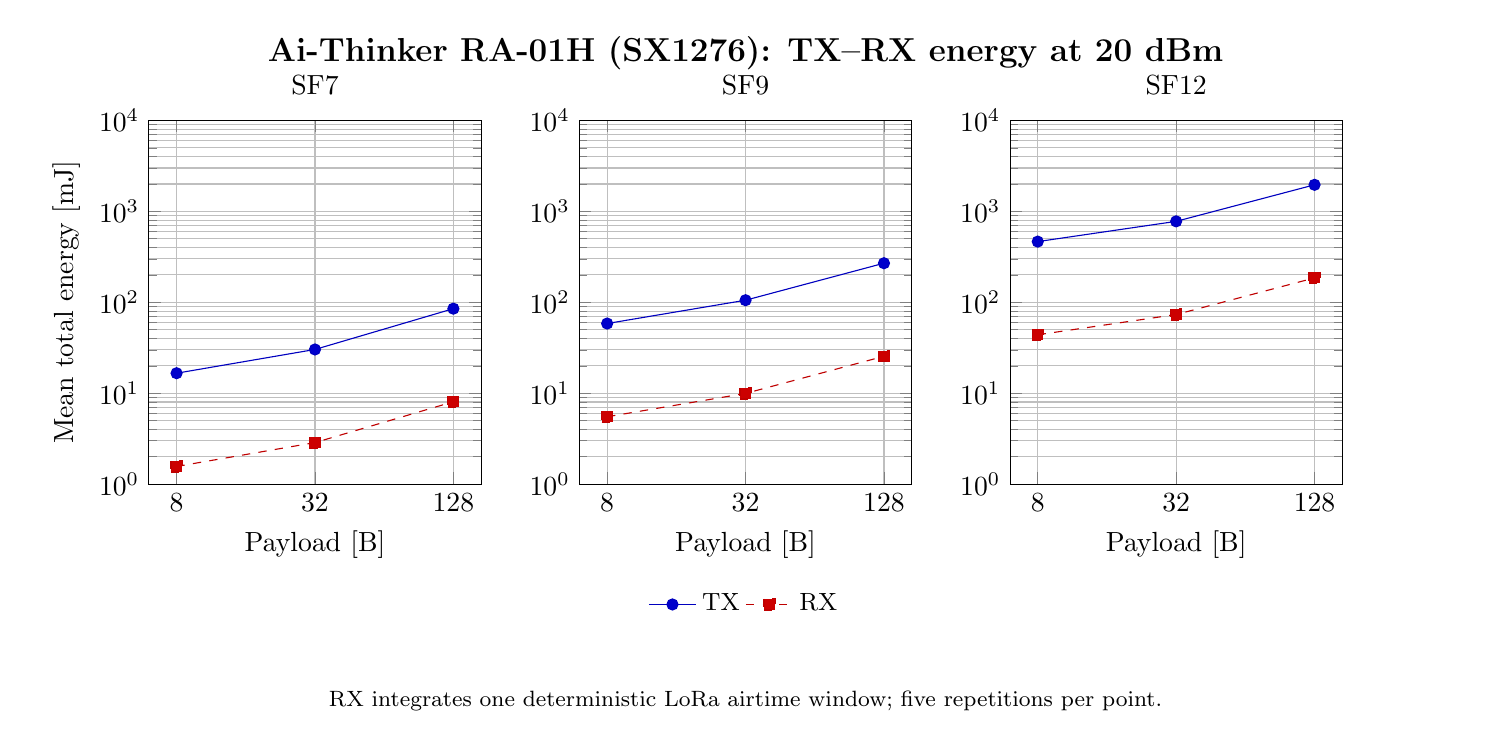
\begin{tikzpicture}
\begin{groupplot}[/pgf/number format/use comma, group style={group size=3 by 1, horizontal sep=1.25cm},
  width=5.8cm,height=6.2cm,xmode=log,log basis x=2,ymode=log,log basis y=10,ymin=1,ymax=10000,
  xtick={8,32,128},xticklabels={8,32,128},grid=both,xlabel={Payload [B]},
  legend style={draw=none,fill=none,font=\small,at={(0.5,-0.27)},anchor=north,legend columns=-1}]
% TX--RX energy
\nextgroupplot[title={SF7},ylabel={Mean total energy [mJ]}]
\addplot+[blue!75!black,solid,mark=*,error bars/.cd,y dir=both,y explicit] coordinates {(8,16.5724889) +- (0,0.0414483964) (32,30.2445219) +- (0,0.0429773056) (128,85.0036059) +- (0,0.236442018)};
\addplot+[red!75!black,dashed,mark=square*,error bars/.cd,y dir=both,y explicit] coordinates {(8,1.56225832) +- (0,0.00261038778) (32,2.85959208) +- (0,0.00224387649) (128,8.04175456) +- (0,0.0137031275)};
\nextgroupplot[title={SF9}]
\addplot+[blue!75!black,solid,mark=*,error bars/.cd,y dir=both,y explicit] coordinates {(8,58.3411324) +- (0,0.137141565) (32,105.308109) +- (0,0.310246775) (128,268.829675) +- (0,0.863137163)};
\addlegendentry{TX}
\addplot+[red!75!black,dashed,mark=square*,error bars/.cd,y dir=both,y explicit] coordinates {(8,5.50195086) +- (0,0.0122728482) (32,9.93646558) +- (0,0.0147846996) (128,25.4370746) +- (0,0.0367928324)};
\addlegendentry{RX}
\nextgroupplot[title={SF12}]
\addplot+[blue!75!black,solid,mark=*,error bars/.cd,y dir=both,y explicit] coordinates {(8,464.664055) +- (0,0.639051593) (32,775.881614) +- (0,0.444753553) (128,1958.53726) +- (0,0.898306677)};
\addplot+[red!75!black,dashed,mark=square*,error bars/.cd,y dir=both,y explicit] coordinates {(8,43.8574712) +- (0,0.0188764315) (32,73.2693061) +- (0,0.0355929547) (128,185.286984) +- (0,0.0688705028)};
\end{groupplot}
\node[font=\bfseries\large] at ($(group c2r1.north)+(0,0.85cm)$) {Ai-Thinker RA-01H (SX1276): TX--RX energy at 20 dBm};
\node[font=\footnotesize,align=center,text width=18cm] at ($(group c2r1.south)+(0,-2.75cm)$) {RX integrates one deterministic LoRa airtime window; five repetitions per point.};
\end{tikzpicture}
\end{document}
